
La plataforma donde desplegar el programa de control ha de disponer de las características necesarias para interactuar con el hardware del  motor de corriente continua y la electrónica de potencia: el puente H\@.
Las soluciones más comerciales son Arduino y Raspberry.
En este tipo de dispositivos se pondrá a prueba la versatilidad de Golang para compilar ejecutables para distintas arquitecturas de chips de forma trasparente para el programador.
Se elige Raspberry como plataforma para albergar el código cliente por poseer una interfaz más amigable de cara al desarrollo y las pruebas del programa.
El ámbito del proyecto ya es lo suficientemente complejo y Arduino pudiera requerir mayor de esfuerzo debido a no disponer de sistema operativo a la hora de trabajar.

En la~\cref{fig:raspberry pins} ilustran los pines disponibles para acceder desde el sistema operativo y en la~\cref{fig:Used Pins} se señalan los utilizados por el programa cliente.

\begin{figure}[H]
    \centering
    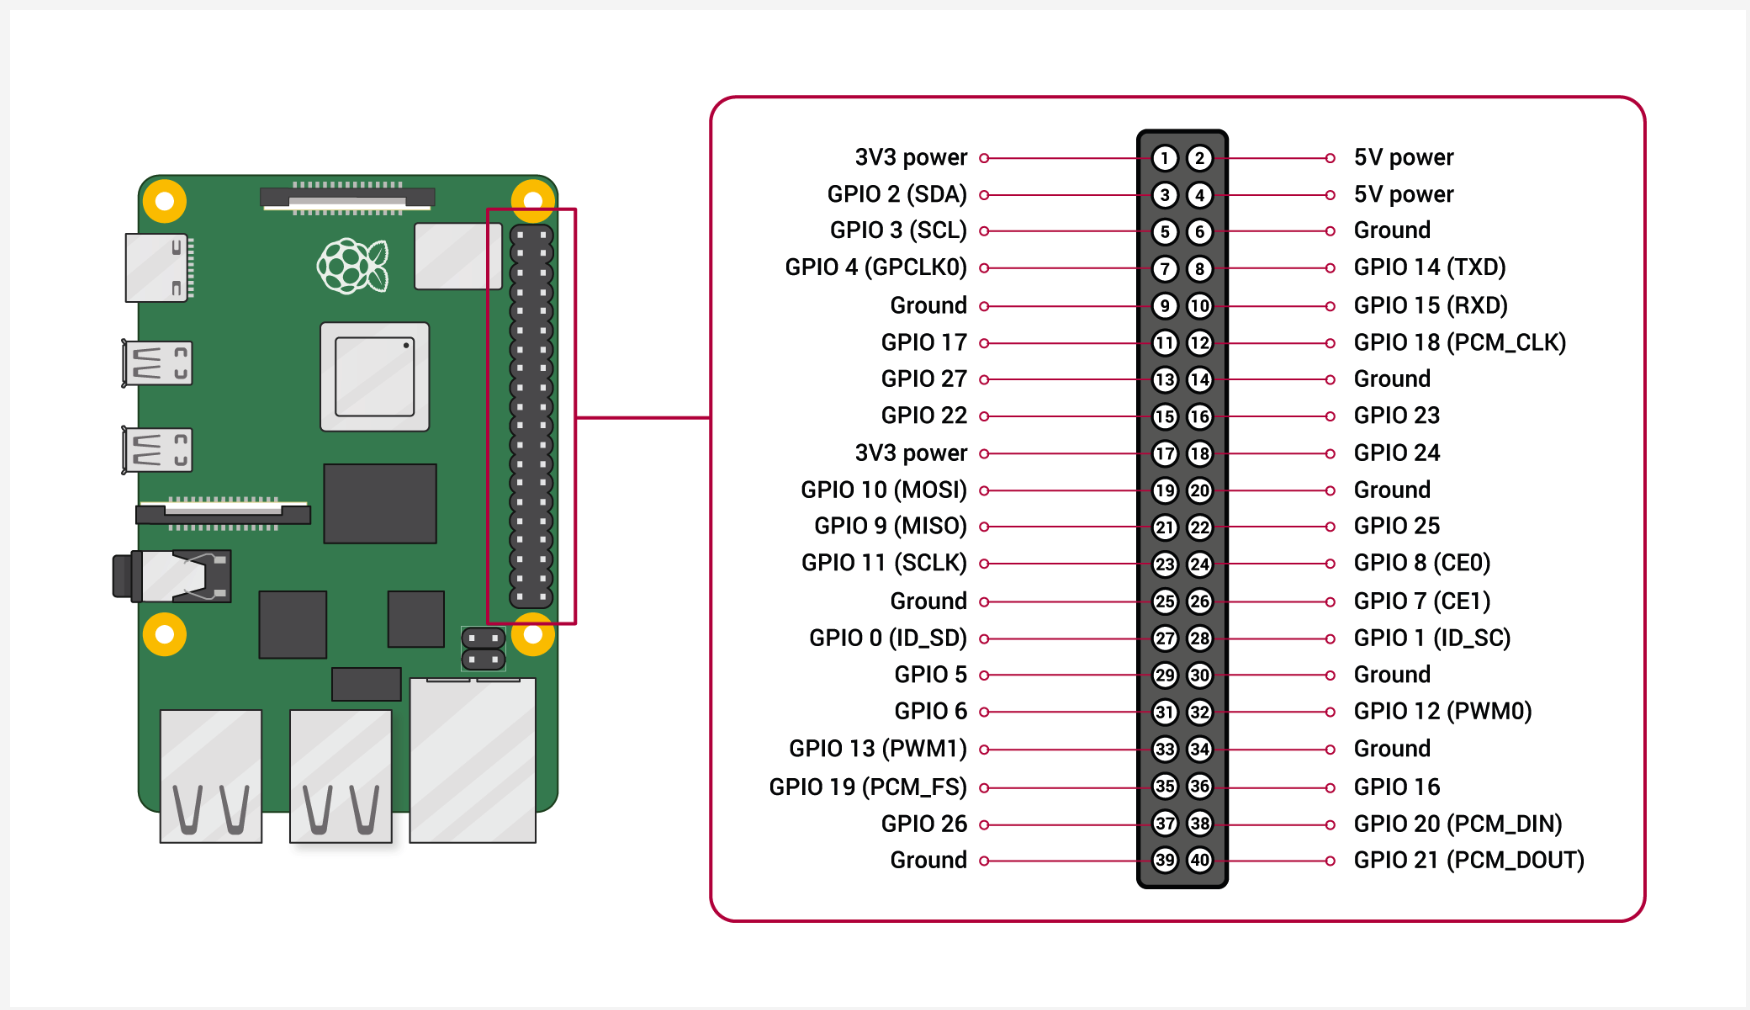
\includegraphics[scale = 0.35]{part/Proyecto_ejecutivo/memoria_constructiva/raspb/img/raspberry}
    \caption{PinSet de Raspberry Pi 4.4\cite{raspberryORG} }\label{fig:raspberry pins}
\end{figure}

\begin{figure}[H]
    \centering
    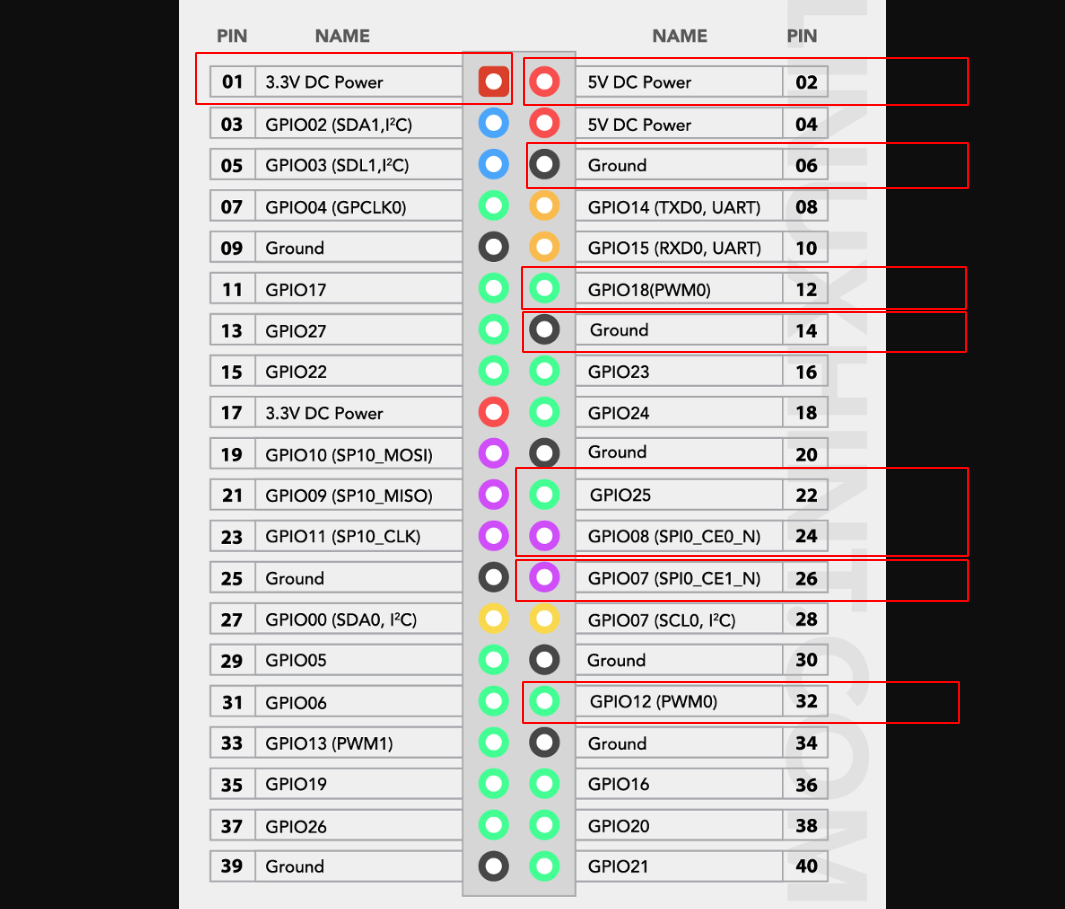
\includegraphics[scale = 0.3]{part/Proyecto_ejecutivo/memoria_constructiva/raspb/img/gpio-pinout-raspberry-pi-01-used}
    \caption{Raspberry: Pins utilizados en el proyecto}\label{fig:Used Pins}
\end{figure}